\scanpage{80}
\mspage{39}
\[
\tag{\unsure{102|107}}
\diagram{\begin{tikzcd}[ampersand replacement=\&, column sep=large,row sep=large]
\& \Pi M^*_{\underline G,\underline G'} \arrow[r] \arrow[d] \& \Pi M_{G'} \\
\Pi(M_{\underline G}\deleted{,\unsure{\Gamma^!_{\underline G,\underline G'}}}) \arrow[r,"\approx"{name=equiv80}] \& \Pi M_{G,G'} \\
\& \begin{gathered}\text{this is an}\\\text{equivalence of}\\\text{groupoids}\end{gathered}
\arrow[from=equiv80,to=3-2,bend right=45]
\end{tikzcd}}
\]
which we are going to rewrite as
\[
\tag{103}
\diagram{\begin{tikzcd}[ampersand replacement=\&, column sep=large,row sep=large]
\Pi M^*_{\underline G,\underline G'} \arrow[r,"\unsure{\gamma_{\underline G,\underline G'}|\psi_{\underline G,\underline G'}}"] \arrow[d,"\varphi_{G,G'}"] \& \Pi M_{G'} \\
\Pi(M_G,\deleted{\unsure{\Gamma^!_{\underline G,\underline G'}}})
\end{tikzcd}}
\]
\margin{``generization diagram for the fundamental groupoids for the quotient of $\underline G\to\underline G'$''}
\deleted{\unsure{but} for what follows, it will be more convenient to write $\Pi M_{G,G'}$ \unsure{in} place of $\Pi(M_G,\unsure{\Gamma^!_{\underline G,\underline G'}})$}

The homomorphism of groupoids $\varphi_{G,G'}$ properties of \deleted{\unsure{the}} the homomorphism on the $\pi_1$ in a fibration with base $(M_G\deleted{,\unsure{\Gamma_{\underline G,\underline G'}}\inserted{\text{actions of }\Gamma^!_{G,G'}}})$, \deleted{with} fiber a product of punctured disks (or circles, if one prefers) --- one can consider $\Pi M^*_{\underline G,\underline G'}$ as a canonical ``\uline{extension}'' of the groupoids $\Pi(M_G,\deleted{\unsure{\Gamma^!_{\underline G,\underline G'}}})$ by
\figure{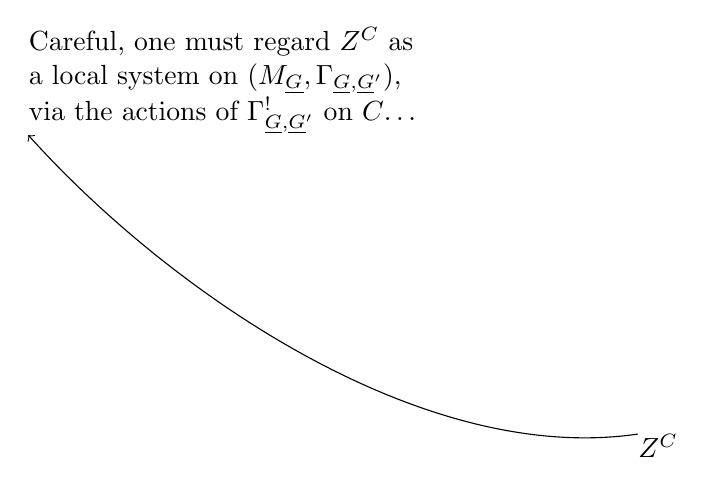
\begin{tikzpicture}[x=1cm,y=1cm]
\node[anchor=base,inner sep=0pt] (z80) at (8,0) {$\mathbb Z^C$};
\node[anchor=south west,align=left,text width=5cm,inner sep=0pt] (attention80) at (0,4.1) {Careful, one must regard $\mathbb Z^C$ as a local system on $(M_{\underline G},\Gamma_{\underline G,\underline G'})$, via the actions of $\Gamma^!_{\underline G,\underline G'}$ on $C$\ldots};
\draw[->] (z80.north west) .. controls (5,-0.1) and (1.8,2.1) .. (attention80.south west);
\end{tikzpicture}}
, where $C$, we recall, is the set of \deleted{\unsure{arrows|boundaries}}\inserted{edges} of $\underline G$
\margin{\uline{NB} $(M_G\deleted{,\unsure{\Gamma_{\underline G,\underline G'}}})$ is a $K(\pi,1)$, and consequently in the exact sequence of the $\pi_1$ of the preceding fibration \unsure{included}, one does indeed have a $1$ on the left}
\margin{79}
